\q{10}{Shoot Your Shot}
\vskip .1in

The \lsi+shots+ table has information for every shot taken (including free throws) in the 2014 - 2015 NBA season. Assume that this table contains information regarding every single point scored in a game this season. 
\lsi+GAME_ID+ is the unique identifier for each game, and each team has a unique three letter code.
\begin{center}
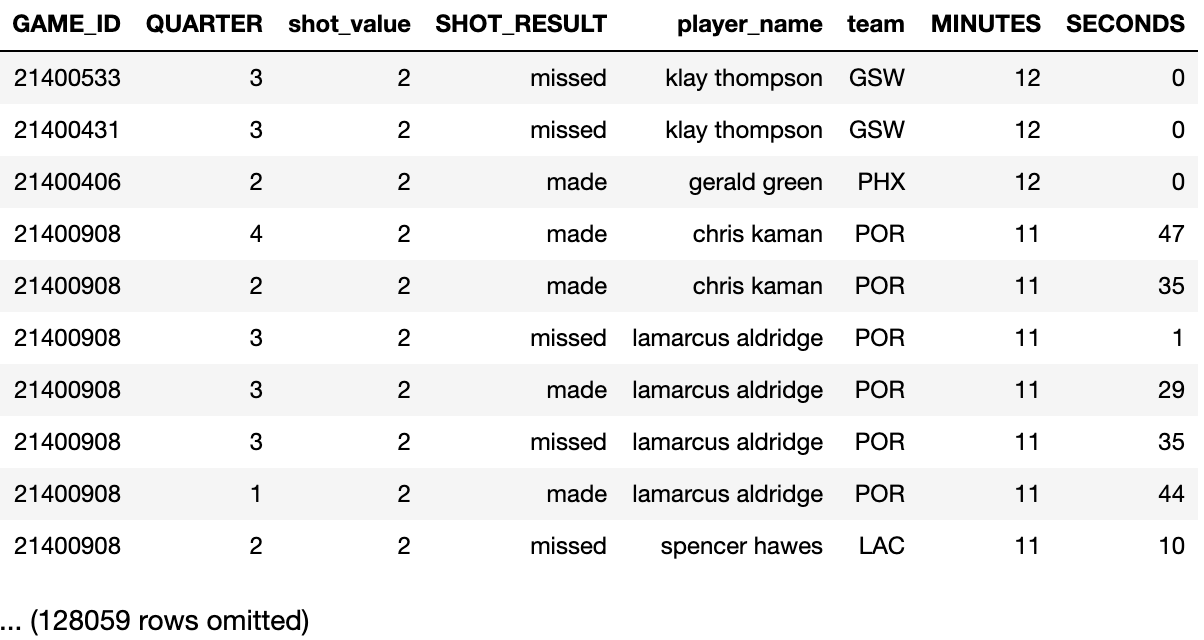
\includegraphics[scale=.6]{figures/shots_table.png}
\end{center}

\begin{enumerate}
\vskip 0.1in
\subq{2}
Write code to produce a table called \lsi+points+ that only contains shots that were "made" (points are only earned if a shot is made in the basket). The resulting table should have three columns: \lsi+GAME_ID+, \lsi+shot_value+, and \lsi+team+.
\vskip .2in
\solutionimage
{
\lstinline+points = shots.+\bklong
}
{
{\lsi+points = shots.where("SHOT_RESULT", are.equal_to("made")).select("GAME_ID", "shot_value", "team")+}
}
\vskip .1in
\subq{2} Assuming the \lsi+points+ table was implemented correctly, write code to produce a table \lsi+scores+ that contains the total number of points scored \textit{per team per game}. 

\vskip .2in
\solutionimage
{
\lstinline+scores = points.+\bkshort+(make_array(+\bkshort+, +\bkshort+), +\bkshort+)+
}
{
{\lsi+scores = points.group(make_array("GAME_ID", "team"), sum)+}
}
\vskip .1in
\subq{2} Assuming the \lsi+scores+ table was implemented correctly, write code to produce a table \lsi+sorted_scores+ where within each game (two rows with the same \lsi+GAME_ID+ but different teams), the row representing the team that scored the most points comes before the row representing the team that scored the least points. 
\vskip .2in
\solutionimage
{
\lstinline+sorted_scores = scores.+\bkshort+(+\bk+, +\bk+).sort("GAME_ID")+
}
{
{\lsi+sorted_scores = scores.sort("shot_value sum", descending = True).sort("GAME_ID")+}
}
\vskip .1in

\subq{4} Assuming the \lsi+sorted_scores+ table was implemented correctly, write code to produce a table called \lsi+win_count+, which should contain two columns:
\begin{itemize}
    \item \lsi+team+: The team name
    \item \lsi+count+: the number of games the team won
\end{itemize}

The team that won the most games should be the first row of the table.\newline
\vskip 0.1in
\solutionimage 
{
\lsi+winners_of_games = sorted_scores.+\bkshort+(np.arange(0,sorted_scores.num_rows,2))+\newline

\lsi+unsorted_winners = winners_of_games.+\bk+(+\bk+)+\newline

\lstinline+win_count = unsorted_winners.+\bk+(+\bk+, +\bk+)+
}
{
{\lsi+winners_of_games = sorted_scores.take(np.arange(0,sorted_scores.num_rows,2))+}\newline
{\lsi+unsorted_winners = winners_of_games.group("team")+}\newline
{\lstinline+win_count = unsorted_winners.sort("count", descending=True)+}

}


\end{enumerate}